\begin{titlepage}
   \begin{center}
       \vspace*{9cm}
       \LARGE
       \textbf{Seguridad 3: Riesgo Eléctrico}
       \vspace{0.8cm}
   \end{center}
\end{titlepage}

\section{Electricidad}
\subsection{Configuración de la red eléctrica}
\begin{enumerate}
    \item % Pregunta 1
La línea monofásica corresponde a un sistema de producción, distribución y consumo de energía que se forma por una sola corriente alterna o una fase. Se compone  de 3 cables: vivo, neutro y de tierra.
\begin{itemize}
    \item \textbf{Vivo:} Denotado por la letra L. Transmite la corriente desde un generador o transformador. Su tensión nominal es de 220 Voltios y su tensión real de 210-223 Voltios. Se identifica por un color azul, negro o rojo. 
    
    \item \textbf{Neutro:} Denotado por la letra N. Corresponde al conductor por donde retorna la corriente. Su tensión nominal es de 0 Voltios con respecto a tierra, y su tensión real de 0-5 Voltios con respecto a tierra. Se identifica por el color blanco.
    
\item \textbf{Tierra de protección:} Denotado por G de ground, o $\Ground$. Corresponde al cable de protección, se usa para para conducir la descarga a tierra de algún artefacto en mal estado. Su tensión nominal es de 0 Voltios. Se identifica por un color verde o verde/amarillo. 
\end{itemize}

 El uso más frecuente de la línea monofásica es la distribución para iluminación, motores eléctricos pequeños y calefacción.
\\ \\
El valor eficaz se usa para comparar una corriente 
\\ \\
La NCh Elec. 4/2003, indica en su artículo 8.0.4.15 que: “Los conductores de una canalización eléctrica se identificarán según el siguiente código de colores:
    \begin{itemize}
        \item \textbf{Conductor de la fase 1:} Azul.
        \item \textbf{Conductor de la fase 2:} Negro.
        \item \textbf{Conductor de la fase 3:} Rojo.
        \item \textbf{Conductor de neutro o tierra de servicio:} Blanco.
        \item \textbf{Conductor de protección:} Verde o Verde/Amarillo.
    \end{itemize}
Fuente: SEC

\item % Pregunta 2
La línea trifásica corresponde a un sistema de producción, distribución y consumo de energía que se forma por tres corrientes alternas monofásicas desfasadas de igual frecuencia y amplitud.
\begin{enumerate}
    \item El voltaje es de 220 Voltios entre fase y tierra. 
    \item El desfase entre las fases es de 120 grados. 
    \item Como el voltaje entre dos fases es 380 Voltios entonces el voltaje rms es $\frac{380}{\sqrt{2}} = 269 \pm 0.3 $ Voltios. 
\end{enumerate}
\newpage

\item % Pregunta 3
Ver figura 1.
\begin{figure}
        \centering
        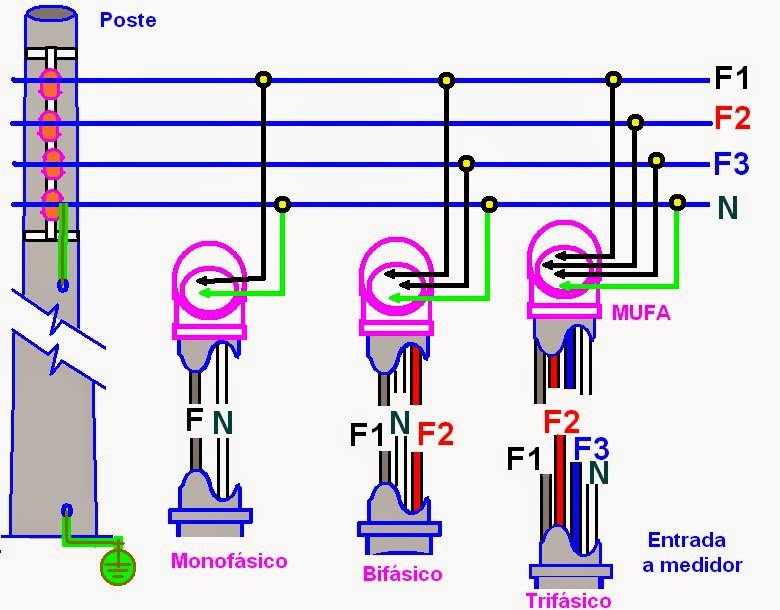
\includegraphics[width=0.7\textwidth]{Imagenes/Seguridad/S3/monofasico-bifasico-y-trifasico.jpg}
        \caption{}
        \label{fig:my_label}
    \end{figure}
\item % Pregunta 4
El interruptor automático es un dispositivo de protección contra sobrecargas y cortocircuitos que tiene la capacidad de actuar cuando detecta la falla sin dañarse, lo cual permite su restablecimiento una vez que se resolvió el inconveniente. Consta de dos mecanismos, uno térmico y otro magnético conectados en serie. Su función es proteger equipos e instalaciones eléctricas.

El mecanismo térmico consiste en una lámina bimetálica que se deforma debido al calor producido por el paso de la corriente. Cuando la corriente es lo suficientemente intensa, la deformación provoca que el circuito se abra interrumpiendo la circulación de corriente. El calentamiento y la deformación del bimetálico son procesos lentos, por eso este mecanismo es apropiado para responde a la sobrecarga de corriente.

El mecanismo magnético consiste en una bobina enrollada sobre un núcleo de material magnético, constituyendo un electroimán. El paso de la corriente produce un campo magnético que desplaza al núcleo del electroimán. Si la corriente es lo bastante intensa, el núcleo acciona el mecanismo y el interruptor se abre. Esto ocurre sin demoras, por lo que este mecanismo es apto para responder a los cortocircuitos.

\item % Pregunta 5
El interruptor diferencial es un aparato capaz de interrumpir o abrir un circuito eléctrico cuando ocurren fallas de aislación en un equipo o instalación eléctrica. Actúa cuando existe una diferencia entre las corrientes entrantes y salientes del circuito. Su función es proteger a las personas. En general están calibradas a 30 mA y su velocidad de respuesta es menor a los 50 ms.

Consiste en un núcleo magnético toroidal al cual están enrolladas la fase y el neutro en sentido contrario mutuamente y además una bobina de detección. Cuando la corriente de entrada es igual a la de salida los campos magnéticos producidos por las bobinas de fase y neutro se anulan, de forma que no hay circulación de corriente en la bobina de detección. Pero si hay alguna fuga a una tierra física, la corriente de entrada y salida no serán iguales, provocando que el campo magnético en el núcleo metálico no sea nulo y produciendo una corriente en la bobina de detección activando un electroimán que abre el circuito.
\item % Pregunta 6
Ver figura \ref{imagenmultiple}.
\begin{images}[\label{imagenmultiple}]{Interruptor diferencial y automático.}
    \addimage[\label{subimagen}]{Imagenes/Seguridad/S3/interruptor diferencial.jpg}{width=7cm}{Interruptor diferencial.}
    \addimage{Imagenes/Seguridad/S3/interruptor automatico.jpg}{width=8cm}{Interruptor automático.}
    
\end{images}
\end{enumerate}
 
\subsection{Efectos Biológicos}
El factor determinante en un accidente eléctrico no es el voltaje aplicado, sino la corriente.
\begin{enumerate}[resume]
     %\setcounter{enumi}{7}
     \item % Pregunta 7
     Los factores primarios, que vendrían siendo los técnicos, corresponden a los que influyen y determinan los efectos de la corriente eléctrica sobre el cuerpo humano. Estos son:
     \begin{itemize}
         \item La cantidad de corriente que fluye sobre a través del cuerpo.
         \item La trayectoria dentro del cuerpo, desde el punto de entrada al de salida.
         \item El tiempo El tiempo durante el cual el cuerpo humano es parte del circuito.
     \end{itemize}
     \item % Pregunta 8
     Los factores secundarios, que vendrían siendo los humanos.
     \begin{itemize}
         \item Edad.
         \item Sexo.
         \item Tamaño y estatura.
         \item Condición física general.
         \item Frecuencia de la corriente.
         \item Piel mojada o transpirada.
     \end{itemize}
     \item % Pregunta 9
     En 1 $cm^2$ de piel seca la resistencia varia entre 15 $k\Omega$ y 1 $M\Omega$. Este valor depende del área de contacto y de la humedad de la piel, en una piel húmeda la resistencia puede bajar hasta el 1\% del valor en la piel seca.
     La resistencia interna del cuerpo es de alrededor de 200 $\Omega$ en los miembros y 500 $\Omega$ en el tronco.
   
     \item % Pregunta 10
     Ver figura \ref{figura pregunta 10}.
     \begin{figure}[H]
         \centering
         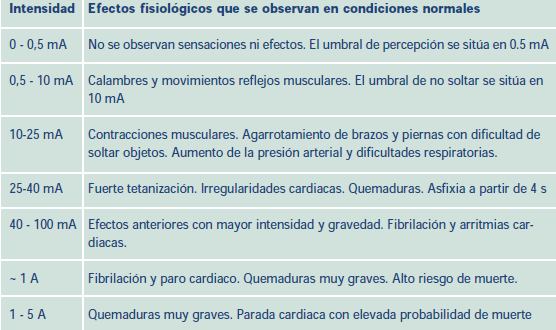
\includegraphics[width=0.6\textwidth]{Imagenes/Seguridad/S3/p10.png}
         \caption{Efectos producidos por el paso de una corriente alterna a una frecuencia de 50/60 Hz. Pregunta 10.}
         \label{figura pregunta 10}
     \end{figure}
     \item % Pregunta 11
     Ver figura \ref{figura pregunta 11}.
     \begin{figure}[H]
         \centering
         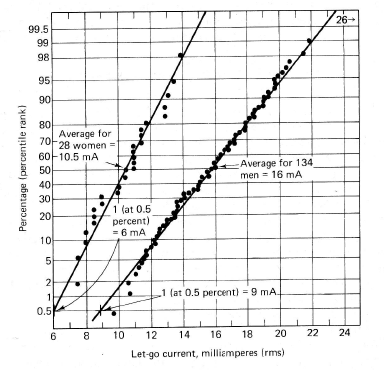
\includegraphics[width=0.7\textwidth]{Imagenes/Seguridad/S3/p11.png}
         \caption{En el gráfico se muestra el umbral de atrapamiento.  La linea izquierda corresponde a mujeres y la derecha corresponde a hombres}
         \label{figura pregunta 11}
     \end{figure}
     
     \item % Pregunta 12
     Ver figura \ref{figura pregunta 12}.
     \begin{figure}[H]
         \centering
         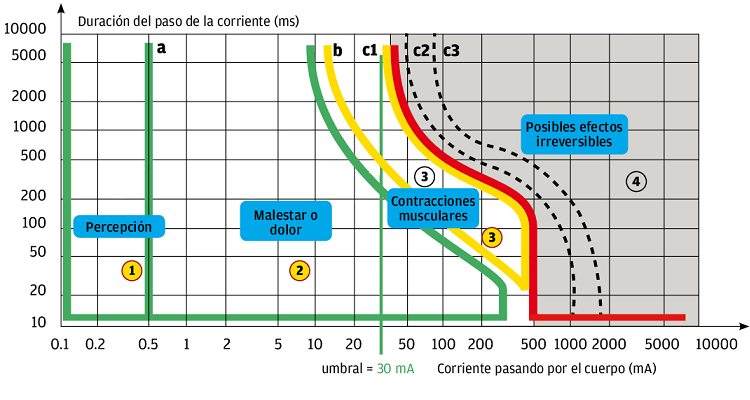
\includegraphics[width=\textwidth]{Imagenes/Seguridad/S3/p12.png}
         \caption{Gráfico ilustrador de la peligrosidad de la corriente con frecuencia.}
         \label{figura pregunta 12}
     \end{figure}
     \begin{itemize}
     
         \item Zona 1: Imperceptible. Generalmente no se perciben efectos con corrientes de hasta 0,5 mA, sin importar el tiempo que esta circule por el cuerpo humano.
         \item Zona 2: Perceptible. Normalmente aún no se producen efectos fisiológicos dañinos. En esta zona se perciben contracciones musculares o tetanizaciones leves.
         \item Zona 3: Efectos reversibles. Por lo general, aún no existe peligro de fibrilación ventricular. En esta zona se pueden producir tetanizaciones y dificultades para la respiración pero que, limitadas en el tiempo, no significan un peligro de muerte.
         \item Zona 4: Posibilidad de efectos irreversibles. Es muy posible que se produzca fibrilación ventricular. El peligro de paro cardiorrespiratorio es alto. Las quemaduras provocadas son graves.
         
     \end{itemize}
     \item % Pregunta 13
     Suponiendo una resistencia de $500\ \Omega$ y que la corriente fatal es de $50 \ mA$ por ley de ohm tenemos,
     \begin{equation}
         V = 5 \cdot 10^{-2} \cdot 500 = 25 \ V
     \end{equation}
     \item % Pregunta 14
        
     \begin{images}[\label{imagenmultiple}]{Umbral de atrapamiento y fibrilación en funcion de la frecuencia.}
         \addimage[\label{subimagen}]{Imagenes/Seguridad/S3/p14_umbral_atrap.jpg}{width=7cm}{Umbral atrapamiento.}
         \addimage{Imagenes/Seguridad/S3/p14_umbral_fibril.jpg}{width=8cm}{Umbral fibrilación.}
    
    \end{images}
    
    El umbral de atrapamiento para una corriente de 50 Hz es de 10 mA y el umbral de fibrilación es de 40 mA.
    Con esto se puede obtener los umbrales para distintas frecuencias de la siguiente forma.
    
    \begin{equation}
        \text{Umbral a la frecuencia estudiada} = F_f \cdot \text{Umbral a la frecuencia de 50 Hz}
    \end{equation}
     
     Como $F_f$ es siempre mayor a uno, se tiene que los umbrales a la frecuencia estudiada son mayores a los umbrales para 50 Hz y por lo tanto las corrientes a mayores frecuencias son menos peligrosas. Sin embargo estas presentan un mayor efecto térmico.
     
     \item % Pregunta 15
     Nunca tocar a la persona para separarla de la fuente. 
     
     Intentar cortar la corriente. Si no es posible hay que intentar separar a la persona utilizando algún elemento que no sea conductor. 
     
     Una vez separada de la fuente se debe evitar mover a la persona. 
     Si hay perdida de conocimiento se debe acostar a la víctima de lado para evitar que se atragante en caso de vomito u otra secreción. Si además la víctima no respira se debe dar asistencia respiratoria. En caso que tampoco haya pulso cardíaco se debe realizar reanimación cardiopulmonar.
     se debe dar aviso a emergencias en caso de 
     \begin{itemize}
         \item quemaduras graves
         \item pérdida de conocimiento
         \item confusión
         \item dificultad para respirar
         \item arritmias o paro cardíaco
         \item dolor y contracciones musculares
         \item convulsiones
     \end{itemize}
     
\end{enumerate}